% Options for packages loaded elsewhere
\PassOptionsToPackage{unicode}{hyperref}
\PassOptionsToPackage{hyphens}{url}
\PassOptionsToPackage{dvipsnames,svgnames,x11names}{xcolor}
%
\documentclass[
  letterpaper,
  DIV=11,
  numbers=noendperiod]{scrreprt}

\usepackage{amsmath,amssymb}
\usepackage{lmodern}
\usepackage{iftex}
\ifPDFTeX
  \usepackage[T1]{fontenc}
  \usepackage[utf8]{inputenc}
  \usepackage{textcomp} % provide euro and other symbols
\else % if luatex or xetex
  \usepackage{unicode-math}
  \defaultfontfeatures{Scale=MatchLowercase}
  \defaultfontfeatures[\rmfamily]{Ligatures=TeX,Scale=1}
\fi
% Use upquote if available, for straight quotes in verbatim environments
\IfFileExists{upquote.sty}{\usepackage{upquote}}{}
\IfFileExists{microtype.sty}{% use microtype if available
  \usepackage[]{microtype}
  \UseMicrotypeSet[protrusion]{basicmath} % disable protrusion for tt fonts
}{}
\makeatletter
\@ifundefined{KOMAClassName}{% if non-KOMA class
  \IfFileExists{parskip.sty}{%
    \usepackage{parskip}
  }{% else
    \setlength{\parindent}{0pt}
    \setlength{\parskip}{6pt plus 2pt minus 1pt}}
}{% if KOMA class
  \KOMAoptions{parskip=half}}
\makeatother
\usepackage{xcolor}
\setlength{\emergencystretch}{3em} % prevent overfull lines
\setcounter{secnumdepth}{5}
% Make \paragraph and \subparagraph free-standing
\ifx\paragraph\undefined\else
  \let\oldparagraph\paragraph
  \renewcommand{\paragraph}[1]{\oldparagraph{#1}\mbox{}}
\fi
\ifx\subparagraph\undefined\else
  \let\oldsubparagraph\subparagraph
  \renewcommand{\subparagraph}[1]{\oldsubparagraph{#1}\mbox{}}
\fi


\providecommand{\tightlist}{%
  \setlength{\itemsep}{0pt}\setlength{\parskip}{0pt}}\usepackage{longtable,booktabs,array}
\usepackage{calc} % for calculating minipage widths
% Correct order of tables after \paragraph or \subparagraph
\usepackage{etoolbox}
\makeatletter
\patchcmd\longtable{\par}{\if@noskipsec\mbox{}\fi\par}{}{}
\makeatother
% Allow footnotes in longtable head/foot
\IfFileExists{footnotehyper.sty}{\usepackage{footnotehyper}}{\usepackage{footnote}}
\makesavenoteenv{longtable}
\usepackage{graphicx}
\makeatletter
\def\maxwidth{\ifdim\Gin@nat@width>\linewidth\linewidth\else\Gin@nat@width\fi}
\def\maxheight{\ifdim\Gin@nat@height>\textheight\textheight\else\Gin@nat@height\fi}
\makeatother
% Scale images if necessary, so that they will not overflow the page
% margins by default, and it is still possible to overwrite the defaults
% using explicit options in \includegraphics[width, height, ...]{}
\setkeys{Gin}{width=\maxwidth,height=\maxheight,keepaspectratio}
% Set default figure placement to htbp
\makeatletter
\def\fps@figure{htbp}
\makeatother
\newlength{\cslhangindent}
\setlength{\cslhangindent}{1.5em}
\newlength{\csllabelwidth}
\setlength{\csllabelwidth}{3em}
\newlength{\cslentryspacingunit} % times entry-spacing
\setlength{\cslentryspacingunit}{\parskip}
\newenvironment{CSLReferences}[2] % #1 hanging-ident, #2 entry spacing
 {% don't indent paragraphs
  \setlength{\parindent}{0pt}
  % turn on hanging indent if param 1 is 1
  \ifodd #1
  \let\oldpar\par
  \def\par{\hangindent=\cslhangindent\oldpar}
  \fi
  % set entry spacing
  \setlength{\parskip}{#2\cslentryspacingunit}
 }%
 {}
\usepackage{calc}
\newcommand{\CSLBlock}[1]{#1\hfill\break}
\newcommand{\CSLLeftMargin}[1]{\parbox[t]{\csllabelwidth}{#1}}
\newcommand{\CSLRightInline}[1]{\parbox[t]{\linewidth - \csllabelwidth}{#1}\break}
\newcommand{\CSLIndent}[1]{\hspace{\cslhangindent}#1}

\KOMAoption{captions}{tableheading}
\makeatletter
\@ifpackageloaded{tcolorbox}{}{\usepackage[many]{tcolorbox}}
\@ifpackageloaded{fontawesome5}{}{\usepackage{fontawesome5}}
\definecolor{quarto-callout-color}{HTML}{909090}
\definecolor{quarto-callout-note-color}{HTML}{0758E5}
\definecolor{quarto-callout-important-color}{HTML}{CC1914}
\definecolor{quarto-callout-warning-color}{HTML}{EB9113}
\definecolor{quarto-callout-tip-color}{HTML}{00A047}
\definecolor{quarto-callout-caution-color}{HTML}{FC5300}
\definecolor{quarto-callout-color-frame}{HTML}{acacac}
\definecolor{quarto-callout-note-color-frame}{HTML}{4582ec}
\definecolor{quarto-callout-important-color-frame}{HTML}{d9534f}
\definecolor{quarto-callout-warning-color-frame}{HTML}{f0ad4e}
\definecolor{quarto-callout-tip-color-frame}{HTML}{02b875}
\definecolor{quarto-callout-caution-color-frame}{HTML}{fd7e14}
\makeatother
\makeatletter
\makeatother
\makeatletter
\@ifpackageloaded{bookmark}{}{\usepackage{bookmark}}
\makeatother
\makeatletter
\@ifpackageloaded{caption}{}{\usepackage{caption}}
\AtBeginDocument{%
\ifdefined\contentsname
  \renewcommand*\contentsname{Table of contents}
\else
  \newcommand\contentsname{Table of contents}
\fi
\ifdefined\listfigurename
  \renewcommand*\listfigurename{List of Figures}
\else
  \newcommand\listfigurename{List of Figures}
\fi
\ifdefined\listtablename
  \renewcommand*\listtablename{List of Tables}
\else
  \newcommand\listtablename{List of Tables}
\fi
\ifdefined\figurename
  \renewcommand*\figurename{Figure}
\else
  \newcommand\figurename{Figure}
\fi
\ifdefined\tablename
  \renewcommand*\tablename{Table}
\else
  \newcommand\tablename{Table}
\fi
}
\@ifpackageloaded{float}{}{\usepackage{float}}
\floatstyle{ruled}
\@ifundefined{c@chapter}{\newfloat{codelisting}{h}{lop}}{\newfloat{codelisting}{h}{lop}[chapter]}
\floatname{codelisting}{Listing}
\newcommand*\listoflistings{\listof{codelisting}{List of Listings}}
\makeatother
\makeatletter
\@ifpackageloaded{caption}{}{\usepackage{caption}}
\@ifpackageloaded{subcaption}{}{\usepackage{subcaption}}
\makeatother
\makeatletter
\@ifpackageloaded{tcolorbox}{}{\usepackage[many]{tcolorbox}}
\makeatother
\makeatletter
\@ifundefined{shadecolor}{\definecolor{shadecolor}{rgb}{.97, .97, .97}}
\makeatother
\makeatletter
\makeatother
\ifLuaTeX
  \usepackage{selnolig}  % disable illegal ligatures
\fi
\IfFileExists{bookmark.sty}{\usepackage{bookmark}}{\usepackage{hyperref}}
\IfFileExists{xurl.sty}{\usepackage{xurl}}{} % add URL line breaks if available
\urlstyle{same} % disable monospaced font for URLs
\hypersetup{
  pdftitle={PHYS2020: Thermoelectric Effects},
  pdfauthor={PHYS2020},
  colorlinks=true,
  linkcolor={blue},
  filecolor={Maroon},
  citecolor={Blue},
  urlcolor={Blue},
  pdfcreator={LaTeX via pandoc}}

\title{PHYS2020: Thermoelectric Effects}
\author{PHYS2020}
\date{}

\begin{document}
\maketitle
\ifdefined\Shaded\renewenvironment{Shaded}{\begin{tcolorbox}[enhanced, boxrule=0pt, borderline west={3pt}{0pt}{shadecolor}, sharp corners, breakable, frame hidden, interior hidden]}{\end{tcolorbox}}\fi

\bookmarksetup{startatroot}

\hypertarget{preface}{%
\chapter*{Preface}\label{preface}}
\addcontentsline{toc}{chapter}{Preface}

\markboth{Preface}{Preface}

These are the laboratory notes for The University of Queensland's
PHYS2020 Thermoelectric Effects experiment.

These notes should be read before attending the lab to maximise time
spent on completing your experiment.

\bookmarksetup{startatroot}

\hypertarget{introduction}{%
\chapter{Introduction}\label{introduction}}

The phenomena linking thermal energy transport and electrical currents
within solid materials are known as the \emph{thermoelectric effects}.
You should already know that electrical currents in a wire follow
\emph{Ohm's law} (Knight 2016)

\begin{equation}\protect\hypertarget{eq-ohms}{}{I = \frac{1}{R}\Delta V}\label{eq-ohms}\end{equation}

where \(I\) is the electrical current intensity, \(R > 0\) is the
electrical resistance of a wire, and \(\Delta V\) is the potential
difference between the endpoints of a wire. Consider a slab of a
conducting materials as shown in Figure~\ref{fig-conductor}.

\begin{figure}

{\centering 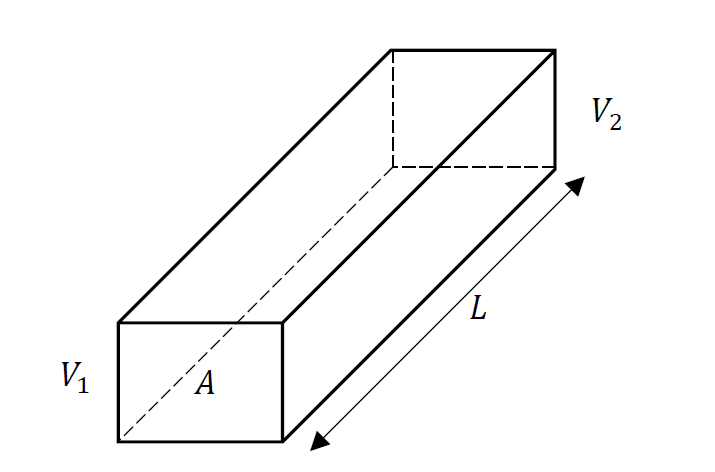
\includegraphics{./images/conductor.png}

}

\caption{\label{fig-conductor}Figure 1: A slab with two ends held at
different electrical potentials.}

\end{figure}

In this case the electrical current can be expressed as

\begin{equation}\protect\hypertarget{eq-current}{}{I = \sigma\frac{A}{L}\Delta V}\label{eq-current}\end{equation}

where \(A\) is the surface area of the slab cross-section, L is its
length, and \(\sigma\) is the electrical conductivity of the material.
The electrical resistance of the slab can be obtained as follows

\begin{equation}\protect\hypertarget{eq-resistance}{}{R = \frac{L}{\sigma A}}\label{eq-resistance}\end{equation}

A similar equation can be obtained for heat transport through the slab.
If the two ends of the slab are kept at different temperatures, the heat
flow \({Q}\) (\({W}\)) is proportional to \(\Delta T\) via(Segrè 2004)

\begin{equation}\protect\hypertarget{eq-heatflow}{}{{Q} = \kappa\frac{A}{L}\Delta T}\label{eq-heatflow}\end{equation}

Where \(\kappa > 0\) is the thermal conductivity (\(Wm^{- 1}K^{- 1}\)),
and \(\Delta T\) is the temperature difference. Note the electrons are
the main carriers of heat and electrical transport in metals. These
similarities hint that there should be a connection between electrical
and thermal currents. This connection is summarised by the
thermoelectric effects. This phenomena has been confirmed
experimentally.

\hypertarget{history}{%
\section{History}\label{history}}

In 1841, James Prescott Joule realised that an electric current has an
inherent thermal effect, called the Joule effect (Martins 2022). Later
in 1851, William Thomson realised that passing an electrical current
through an unequally heated conductor released or absorbed heat
depending on the direction of the heat and electrical currents and the
type of material (Thomson 1856). The irreversible Joule effect is about
two orders of magnitude larger than the reversible Thomson effect, but
both occur simultaneously while a current passes through a material
(Macia 2015). These thermoelectric effects make up the backbone for how
we got to heat engines and heat pumps from thermoelectric materials.

It was Thomas Johann Seebeck who first observed that if you connect
three homogenous conductors connected in series, each at a different
temperature, an electric current flows around the closed circuit (Engel
and Reid 2013). The circuit is known as thermoelectric (TE) circuit.
Hence, the \emph{Seebeck effect} describes the conversion of thermal
energy into electrical energy in the form of an electrical current.

The \emph{Seebeck Voltage} \(\Delta V_{S}\) of a TE circuit is
proportional to the temperature difference of \(T_{H}\) and \(T_{C}\)
(Macia 2015)

\begin{equation}\protect\hypertarget{eq-seebeckV}{}{\Delta V_{s} = S\Delta T}\label{eq-seebeckV}\end{equation}

where \(S(T)\) is a temperature dependent property of the junction
materials, with units \(VK^{- 1}\).

Jean Charles Peltier reported that passing a current across a junction
at thermal equilibrium caused it to absorb heat from the surroundings
\(\left( \Delta Q_{P} < 0 \right)\), while if you reversed the current
the junction released heat to the environment
\(\left( \Delta Q_{P} < 0 \right)\) (Segrè 2004). This \emph{Peltier
Effect} was illustrated nicely by Friedrich Emil Lenz in 1838, who
placed a drop of water on the junction of bismuth and antimony wires
(Macia 2015). When Lenz passed a current through the junction, the water
froze; then when Lenz reversed the current, the ice melted. This was the
first demonstration of TE refrigeration. The \emph{Peltier Heat} is
proportional to current \(I\), duration \(\Delta t\) of the current
applied via

\begin{equation}\protect\hypertarget{eq-peltierH}{}{\Delta Q_{P} = \Pi(T)I\Delta t}\label{eq-peltierH}\end{equation}

Where \(\Pi(T)\) is called the Peltier coefficient (Engel and Reid
2013).

\bookmarksetup{startatroot}

\hypertarget{thermoelectric-devices}{%
\chapter{Thermoelectric Devices}\label{thermoelectric-devices}}

Thermoelectric devices are small, solid-state devices used in
small-scale power generation and refrigeration applications. A thermal
gradient generates an electric current (TE generator, TEG) or a DC
current is applied to remove heat from the cold side (TE cooler, TEC).
Thermoelectric devices generally consist of a relative large number of
thermocouples associated electrically in series and thermally in
parallel.

\begin{figure}

{\centering 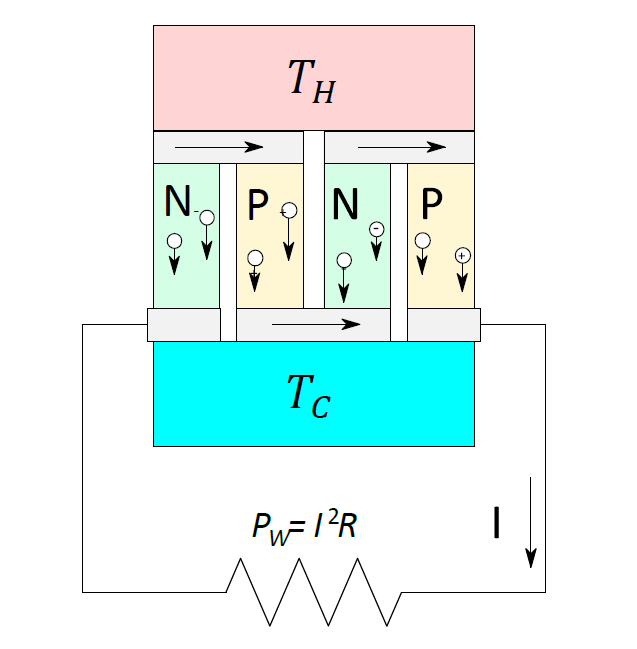
\includegraphics{./images/thermocouple.png}

}

\caption{\label{fig-thermocouple}A thermoelectric generator made of two
thermocouples}

\end{figure}

\begin{tcolorbox}[enhanced jigsaw, toprule=.15mm, coltitle=black, bottomrule=.15mm, colbacktitle=quarto-callout-tip-color!10!white, opacitybacktitle=0.6, titlerule=0mm, colframe=quarto-callout-tip-color-frame, title=\textcolor{quarto-callout-tip-color}{\faLightbulb}\hspace{0.5em}{Question 1}, leftrule=.75mm, bottomtitle=1mm, breakable, opacityback=0, arc=.35mm, left=2mm, colback=white, rightrule=.15mm, toptitle=1mm]

Where would you find TECs/TEGs in practice? What are the advantages of
TE devices compared to other energy technologies? What are their
drawbacks? Note: include your answer in the Introduction/Theory

\end{tcolorbox}

A thermocouple is formed by a n-type and a p-type thermoelement (in what
is a called a leg or branch). A n-type leg or branch has length
\(L_{n}\) and cross-section \(A_{n}\). The two legs are connected by a
conductor at the hot end (\(T_{H}\)) that is assumed to have negligible
electrical and thermal resistance. To close the circuit a load resistor,
with a resistance \(R\), is connected between the cold end of the
thermoelements (\(T_{C}\)).

The temperature difference \(T_{H} - T_{C} \equiv \Delta T > 0\)
generates the Seebeck Voltage
\(\Delta V = \left( S_{p} - S_{n} \right)\Delta T\) at the hot junction,
where \(S_{p} > 0\) and \(S_{n} < 0\) are the Seebeck coefficients of
the p-type and n-type thermoelements, respectively (Macia 2015; Engel
and Reid 2013). The internal electrical resistance of the thermopile
shown in Figure~\ref{fig-thermocouple} is

\begin{equation}\protect\hypertarget{eq-restherm}{}{r = 2\left( \frac{L_{n}}{\sigma_{n}A_{n}} + \frac{L_{p}}{\sigma_{p}A_{p}} \right)}\label{eq-restherm}\end{equation}

where \(\sigma_{n}\) and \(\sigma_{p}\) are the legs conductivities.

\begin{tcolorbox}[enhanced jigsaw, toprule=.15mm, coltitle=black, bottomrule=.15mm, colbacktitle=quarto-callout-tip-color!10!white, opacitybacktitle=0.6, titlerule=0mm, colframe=quarto-callout-tip-color-frame, title=\textcolor{quarto-callout-tip-color}{\faLightbulb}\hspace{0.5em}{Question 2}, leftrule=.75mm, bottomtitle=1mm, breakable, opacityback=0, arc=.35mm, left=2mm, colback=white, rightrule=.15mm, toptitle=1mm]

Explain how Equation~\ref{eq-restherm} has been derived. You need to
recall connection of resistors in series and in parallel.

\end{tcolorbox}

From an electrical point of view, a thermoelectric generator can be
replaced with a voltage source and a resistor in series. Therefore, the
entire device shown in Figure 2 is equivalent to the electric circuit
shown in Figure~\ref{fig-circuit}.

\begin{figure}

{\centering 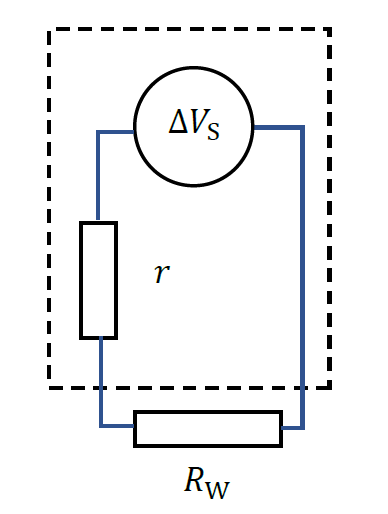
\includegraphics{./images/circuit.png}

}

\caption{\label{fig-circuit}Equivalent electrical circuit for a
thermoelectric generator.}

\end{figure}

The electrical current in the circuit is

\begin{equation}\protect\hypertarget{eq-currentT}{}{I = \frac{\Delta V_{S}}{r + R}}\label{eq-currentT}\end{equation}

\begin{tcolorbox}[enhanced jigsaw, toprule=.15mm, coltitle=black, bottomrule=.15mm, colbacktitle=quarto-callout-tip-color!10!white, opacitybacktitle=0.6, titlerule=0mm, colframe=quarto-callout-tip-color-frame, title=\textcolor{quarto-callout-tip-color}{\faLightbulb}\hspace{0.5em}{Question 3}, leftrule=.75mm, bottomtitle=1mm, breakable, opacityback=0, arc=.35mm, left=2mm, colback=white, rightrule=.15mm, toptitle=1mm]

Explain how Equation~\ref{eq-currentT} is obtained.

\end{tcolorbox}

The power delivered to external load is given by

\begin{equation}\protect\hypertarget{eq-power}{}{W = \frac{{\Delta V_{S}^{2}}R}{(r + R)^{2}}}\label{eq-power}\end{equation}

This can also be written as

\begin{equation}\protect\hypertarget{eq-poweral}{}{W = I\Delta V_{S} - rI^{2}}\label{eq-poweral}\end{equation}

where the first term can be interpreted as the electric power due to the
Seebeck effect, and the second term is the power lost by Joule heating
due to the internal resistance.

\begin{tcolorbox}[enhanced jigsaw, toprule=.15mm, coltitle=black, bottomrule=.15mm, colbacktitle=quarto-callout-tip-color!10!white, opacitybacktitle=0.6, titlerule=0mm, colframe=quarto-callout-tip-color-frame, title=\textcolor{quarto-callout-tip-color}{\faLightbulb}\hspace{0.5em}{Question 4}, leftrule=.75mm, bottomtitle=1mm, breakable, opacityback=0, arc=.35mm, left=2mm, colback=white, rightrule=.15mm, toptitle=1mm]

Recall how to calculate electrical power delivered to a resistor (this
electrical power is converted back to heat but if the resistor is
replaced by an electrical motor, it can be converted into work) and
derive Equation~\ref{eq-power} and obtain Equation~\ref{eq-poweral}.

\end{tcolorbox}

\begin{tcolorbox}[enhanced jigsaw, toprule=.15mm, coltitle=black, bottomrule=.15mm, colbacktitle=quarto-callout-tip-color!10!white, opacitybacktitle=0.6, titlerule=0mm, colframe=quarto-callout-tip-color-frame, title=\textcolor{quarto-callout-tip-color}{\faLightbulb}\hspace{0.5em}{Question 5}, leftrule=.75mm, bottomtitle=1mm, breakable, opacityback=0, arc=.35mm, left=2mm, colback=white, rightrule=.15mm, toptitle=1mm]

Use what you have learned in calculus about finding a maximum (minimum)
of a function and obtain the maximum output power for a TE device.

\end{tcolorbox}

\begin{tcolorbox}[enhanced jigsaw, toprule=.15mm, coltitle=black, bottomrule=.15mm, colbacktitle=quarto-callout-tip-color!10!white, opacitybacktitle=0.6, titlerule=0mm, colframe=quarto-callout-tip-color-frame, title=\textcolor{quarto-callout-tip-color}{\faLightbulb}\hspace{0.5em}{Question 6}, leftrule=.75mm, bottomtitle=1mm, breakable, opacityback=0, arc=.35mm, left=2mm, colback=white, rightrule=.15mm, toptitle=1mm]

Assuming symmetry between thermocouple legs, derive the maximum output
power in terms of the design parameters \(A,\ L\).

\end{tcolorbox}

\hypertarget{thermoelectric-efficiency}{%
\section{Thermoelectric Efficiency}\label{thermoelectric-efficiency}}

In this experiment, all measurements will be in terms of power rather
than energy. A thermoelectric generator is a type of heat engine, which
means the efficiency is defined by the ratio

\[\eta = \frac{W}{\dot{Q}_{H}}\]

where \(W\) is the power delivered to the external load and
\(\dot{Q}_{H}\) is the heat power (measured in W) entering the hot
junction (source). However, some heat exits the engine at the cold
junction (sink).

The overall Heat power \(\dot{Q}_{H} = \dot{Q}_{P} + \dot{Q}_{n}\) can
be expressed in the form

\[\dot{Q}_{H}= IT_{H}\left( S_{p} - S_{n} \right) + \kappa\Delta T - \frac{I^{2}}{2}r\]

where the first term is the reversible heat release, and the last two
terms are irreversible: Fourier diffusion and the Joule effect.

\begin{tcolorbox}[enhanced jigsaw, toprule=.15mm, coltitle=black, bottomrule=.15mm, colbacktitle=quarto-callout-tip-color!10!white, opacitybacktitle=0.6, titlerule=0mm, colframe=quarto-callout-tip-color-frame, title=\textcolor{quarto-callout-tip-color}{\faLightbulb}\hspace{0.5em}{Question 7 (Advanced)}, leftrule=.75mm, bottomtitle=1mm, breakable, opacityback=0, arc=.35mm, left=2mm, colback=white, rightrule=.15mm, toptitle=1mm]

Assume there are no irreversible effects, show that the expression
\(\eta = W/\dot{Q}_{H}\) will reduce to the Carnot limit
\(\eta_{c} = \Delta T/T_{H}\).

\end{tcolorbox}

A thermoelectric cooler's performance can be analysed in a similar way
to TEGs (as above). The difference lies in an external battery driving
the electrons in the n-type leg and holes in the p-type leg away from
the cold junction to the hot one. Hence, the heat power is determined by
the opposite contributions stemming from Fourier flow and the Peltier
effect. The electric power \(W_{C}\ \)consumed by the battery feeding
the thermocouple is given by

\[W_{C} = I\Delta V + rI^{2}\]

The efficiency is expressed in terms of the coefficient of performance
(COP)

\[\phi = \frac{Q_{C}}{W_{C}}\]

Note a COP of 0 is the maximum cooling temperature difference a TEC can
reach. A COP of infinity is the theoretical maximum efficiency.

\bookmarksetup{startatroot}

\hypertarget{experiment}{%
\chapter{Experiment}\label{experiment}}

Your assignment is to investigate the thermoelectric effects -- Seebeck
and Peltier -- and write a lab report on your findings. You will be
required to come up with your own experiment. However, it is recommended
to follow through the guided exploration below first.

The experiment has two parts: the heat engine (Seebeck) and heat pump
(Peltier).

This experiment uses the following equipment:

\begin{itemize}
\item
  Peltier device
\item
  Alpha immersion thermostat w/ thermal bath
\item
  Two thermometers
\item
  4 multimeters
\item
  A power supply capable of running 0V → 18V DC (max current 5A) and
  stepped-down 2V → 15V AC voltage (max current 5A) simultaneously
\item
  A variable resistor (0Ω → 33Ω)
\item
  A basic resistor breadboard
\item
  Assorted resistors: (1.0 ± 2\%) Ω, (2.0 ± 2\%) Ω, (5.0 ± 5\%) Ω, and
  (10.0 ± 2\%) Ω
\item
  Cables
\end{itemize}

\hypertarget{power-supply}{%
\section{Power supply}\label{power-supply}}

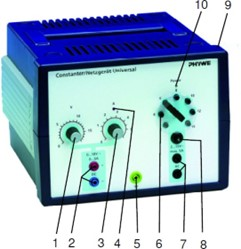
\includegraphics{./images/PowerSupply.jpg}

\begin{enumerate}
\def\labelenumi{\arabic{enumi}.}
\item
  (DC) Voltage adjustment knob
\item
  \begin{enumerate}
  \def\labelenumii{(\Roman{enumii})}
  \setcounter{enumii}{599}
  \tightlist
  \item
    Output
  \end{enumerate}
\item
  (DC) Current limiter knob
\item
  Indicator light - operating at maxi- mum limited current
\item
  Earthed lead
\item
  (AC) Selection of voltage step
\item
  (AC) Output
\item
  (AC) Overload circuit breaker
\item
  On/off switch and fuse holder
\item
  Operation indicator light
\end{enumerate}

\begin{tcolorbox}[enhanced jigsaw, toprule=.15mm, coltitle=black, bottomrule=.15mm, colbacktitle=quarto-callout-important-color!10!white, opacitybacktitle=0.6, titlerule=0mm, colframe=quarto-callout-important-color-frame, title=\textcolor{quarto-callout-important-color}{\faExclamation}\hspace{0.5em}{Warning}, leftrule=.75mm, bottomtitle=1mm, breakable, opacityback=0, arc=.35mm, left=2mm, colback=white, rightrule=.15mm, toptitle=1mm]

The DC output of the power supply must only be used as an input for the
Peltier Device. The AC output of the power supply must only be used as
an input for the heating coil (maximum 4 V). To change the AC output,
use the rheostat to change the reistance according to \(V=IR%
\).

\end{tcolorbox}

\hypertarget{alpha-immersion-thermostat}{%
\section{Alpha immersion thermostat}\label{alpha-immersion-thermostat}}

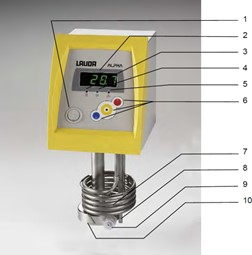
\includegraphics{./images/Thermostat.jpg}

\begin{enumerate}
\def\labelenumi{\arabic{enumi}.}
\item
  Power Switch
\item
  Temperature controller with four segment LED display
\item
  Heater indicator light (yellow LED)
\item
  Cooler indicator light (blue LED)
\item
  Error indicator light (red LED)
\item
  Menu functions, select and enter keys
\item
  Tubular heater
\item
  Temperature probe Pt100
\item
  Pump outflow or pressure outlet with pump outflow reducer
\item
  Pump housing
\end{enumerate}

\begin{tcolorbox}[enhanced jigsaw, toprule=.15mm, coltitle=black, bottomrule=.15mm, colbacktitle=quarto-callout-important-color!10!white, opacitybacktitle=0.6, titlerule=0mm, colframe=quarto-callout-important-color-frame, title=\textcolor{quarto-callout-important-color}{\faExclamation}\hspace{0.5em}{Warning}, leftrule=.75mm, bottomtitle=1mm, breakable, opacityback=0, arc=.35mm, left=2mm, colback=white, rightrule=.15mm, toptitle=1mm]

Because the thermostat is used as the hot reservoir (up to 80°C), please
exercise caution to avoid burning yourself. Wear the provided gloves if
handling any of the heated-up equipment.

\end{tcolorbox}

\hypertarget{peltier-experiment-apparatus}{%
\section{Peltier Experiment
Apparatus}\label{peltier-experiment-apparatus}}

\begin{figure}

{\centering 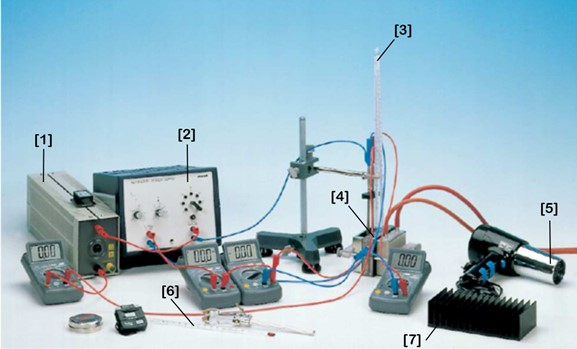
\includegraphics{./images/PeltierApparatus.jpg}

}

\caption{\label{fig-apparatus}This figure displays the setup for the
Peltier (cooling) Experiment}

\end{figure}

\begin{enumerate}
\def\labelenumi{\arabic{enumi}.}
\item
  Variable resistor
\item
  Power supply
\item
  Thermometer (slots into Peltier device holes)
\item
  Peltier device (Thermoelectric device)
\item
  Blower
\item
  Second thermometer (can sit in reservoir of still water)
\item
  Heat sink
\end{enumerate}

\begin{tcolorbox}[enhanced jigsaw, toprule=.15mm, coltitle=black, bottomrule=.15mm, colbacktitle=quarto-callout-important-color!10!white, opacitybacktitle=0.6, titlerule=0mm, colframe=quarto-callout-important-color-frame, title=\textcolor{quarto-callout-important-color}{\faExclamation}\hspace{0.5em}{Warning}, leftrule=.75mm, bottomtitle=1mm, breakable, opacityback=0, arc=.35mm, left=2mm, colback=white, rightrule=.15mm, toptitle=1mm]

To keep yourself safe and the equipment undamaged, please consult with
the tutors before turning on any of the equipment.

\end{tcolorbox}

\bookmarksetup{startatroot}

\hypertarget{guided-exploration}{%
\chapter{Guided Exploration}\label{guided-exploration}}

\hypertarget{thermoelectric-generator-teg}{%
\section{Thermoelectric Generator
(TEG)}\label{thermoelectric-generator-teg}}

To start, we'll be looking at a thermoelectric generator (heat engine).
In other words, we will look at how much electrical energy (power) is
produced from the thermoelectric device at varying temperature
differences of \(T_{H}\) and \(T_{C}\).

Connect the Thermostat water bath to the TEG device, making sure that
the black covering (on the TEG) is flush with the metal water container
as to not leak water. Place both thermometers into the designated
\(T_{H}\) and \(T_{C}\) holes (add thermo-paste into the hole for better
thermal contact). Then connect a voltmeter (in parallel) and an ammeter
(in series). Turn on the thermostat (hot reservoir) and allow for water
to be pumped into the TEG. Also turn on the water pump in the large
barrel. Both the cold reservoir (from the water barrel) and hot
reservoir (thermostat bath) should be at room temperature to start.
Note, if any, electrical energy is being produced from the TEG at
\(\Delta T \approx 0\).

Let's first find the Seebeck coefficient. To do this, we will need to
run our circuit \textbf{without} a load resistor. This circuit has
approximately zero resistance.

\begin{tcolorbox}[enhanced jigsaw, toprule=.15mm, coltitle=black, bottomrule=.15mm, colbacktitle=quarto-callout-note-color!10!white, opacitybacktitle=0.6, titlerule=0mm, colframe=quarto-callout-note-color-frame, title={Task 1}, leftrule=.75mm, bottomtitle=1mm, breakable, opacityback=0, arc=.35mm, left=2mm, colback=white, rightrule=.15mm, toptitle=1mm]

Measure the no-load voltage and short-circuit current of the circuit
(without a load resistor) at varying temperature differences up to
\(T_{H} = 60{^\circ}C\). Find the Seebeck coefficient of the
semiconductor combination (Hint: there are 142 thermocouple elements
connected in series within the device). You must include uncertainty
propagation and an evaluation of your result. After plotting the
measurements, what does this relationship tell us about the internal
resistance of the TEG device? (Hint: consider Ohm's law).

\end{tcolorbox}

Next, we will connect the rheostat (load resistor) with resistance \(R\)
to the TEG (or the breadboard if you're comfortable with it). Our goal
here is to find the value of the internal resistance of the TEG device.
The thermostat temperature should still be at \(60{^\circ}\)C from the
previous task. While not necessary for this part, it is a good idea to
know what resistance your rheostat is set to at each measurement.
However, we will only be measuring current and voltage here.

\begin{tcolorbox}[enhanced jigsaw, toprule=.15mm, coltitle=black, bottomrule=.15mm, colbacktitle=quarto-callout-note-color!10!white, opacitybacktitle=0.6, titlerule=0mm, colframe=quarto-callout-note-color-frame, title={Task 2}, leftrule=.75mm, bottomtitle=1mm, breakable, opacityback=0, arc=.35mm, left=2mm, colback=white, rightrule=.15mm, toptitle=1mm]

Measure the voltage and current of the circuit at a constant temperature
difference (record your error/uncertainty) at different load
resistances. Find the maximum Seebeck voltage \(V(I = 0)\), available at
this temperature difference and the short circuit current
\(I_{s}(V = 0)\), as well as the internal resistance of the TEG device.
Propagate your uncertainties.

\end{tcolorbox}

Finally, we will be calculating the heat \(\dot{Q}_{H}\) flowing through
the generator in unit time according to
\(\frac{dQ}{dt} = \dot{Q}_{H} = m_{w}c_{w}\left( \frac{d\Delta T}{dt} \right)\).
And we'll also calculate the electrical power, measured at constant
load, \(W\). You will need to estimate the mass of the water \(m_{w}\)
in the container.

\begin{tcolorbox}[enhanced jigsaw, toprule=.15mm, coltitle=black, bottomrule=.15mm, colbacktitle=quarto-callout-note-color!10!white, opacitybacktitle=0.6, titlerule=0mm, colframe=quarto-callout-note-color-frame, title={Task 3}, leftrule=.75mm, bottomtitle=1mm, breakable, opacityback=0, arc=.35mm, left=2mm, colback=white, rightrule=.15mm, toptitle=1mm]

Set the Rheostat resistance to equal the internal resistance of the TEG
device (you found in Task 2). Record the temperature of both sides of
the TEG device over time as you go from \(60{^\circ}C\) to
\(80{^\circ}C\). Then turn off the thermostat heat bath and continue
recording the temperature for the next 10-15 minutes as it cools. Record
the current and voltage output at each increment too. Find the maximum
efficiency \(\eta^{*}\).

\end{tcolorbox}

Summary: We've observed how a thermoelectric device has operated as a
heat engine. We've calculated the Seebeck Coefficient, the internal
resistance of the TEG device, and used it to find the maximum efficiency
of the device. We should know what properties a TEG device should have
to run at an optimal level and what its drawbacks are.

\hypertarget{thermoelectric-cooler-tec}{%
\section{Thermoelectric Cooler (TEC)}\label{thermoelectric-cooler-tec}}

First, let's figure out which way we need to pass the current through
the TEC to make it cool the correct side. Fix the water container with
the hole in the top (for the heating coil) instead of the thermostat
container. Fill it with room temperature water. Connect the TEC device
to the power supply through the DC side. Turn it on. You should now see
on the thermometers which side is heating up and which side is cooling
down. Swap the positive/negative cables to make the heating-coil side
cool down.

Now add the heating coil (\(R_{coil} \approx 3\Omega\)) to the water
container. Make sure it is submerged in the water and not touching the
sides before turning it on. It must be connected to the AC and not
higher than 3.5 A of current.

Our goal is to calculate the cooling capacity \(\dot{Q}_{C}\). A nifty
way to do this is to match the cooling capacity with the heating of the
coil. This means that the cooling effect of the Peltier is balancing out
the heating of the coil. Hence, the temperature of both sides shouldn't
change.

\begin{tcolorbox}[enhanced jigsaw, toprule=.15mm, coltitle=black, bottomrule=.15mm, colbacktitle=quarto-callout-note-color!10!white, opacitybacktitle=0.6, titlerule=0mm, colframe=quarto-callout-note-color-frame, title={Task 4}, leftrule=.75mm, bottomtitle=1mm, breakable, opacityback=0, arc=.35mm, left=2mm, colback=white, rightrule=.15mm, toptitle=1mm]

Match the heating output of the heating coil with the cooling output of
the TEC at multiple TEC current inputs, i.e., set the input DC current
of the cooling device; match the heating coil input to achieve zero
temperature difference by changing the resistance of the rheostat.
Measure the heater current and voltage, the operating current and
voltage, and the temperatures \(T_{H}\) and \(T_{C}\). Find the COP
\(\phi\) at multiple input DC currents.

\end{tcolorbox}

\begin{tcolorbox}[enhanced jigsaw, toprule=.15mm, coltitle=black, bottomrule=.15mm, colbacktitle=quarto-callout-warning-color!10!white, opacitybacktitle=0.6, titlerule=0mm, colframe=quarto-callout-warning-color-frame, title=\textcolor{quarto-callout-warning-color}{\faExclamationTriangle}\hspace{0.5em}{Note}, leftrule=.75mm, bottomtitle=1mm, breakable, opacityback=0, arc=.35mm, left=2mm, colback=white, rightrule=.15mm, toptitle=1mm]

Students should check their progress with their tutors before proceeding
any further.

\end{tcolorbox}

\bookmarksetup{startatroot}

\hypertarget{your-own-experiment}{%
\chapter{Your own experiment}\label{your-own-experiment}}

Take some time now to formulate what your own investigation will be.
Discuss your plans with a tutor before you start. Here are two example
extensions to focus on; however, you are welcome to propose your own
experiment to the tutors.

\hypertarget{heating-and-cooling-efficiency}{%
\section{Heating and Cooling
Efficiency}\label{heating-and-cooling-efficiency}}

If you run the apparatus as a heat pump, you could investigate the
maximum coefficient of performance that could be achieved, and what the
main factors that limit this performance. To measure the COP, you will
need to find a way to measure the power extracted from the cold
reservoir or added to the hot reservoir (depending on whether you are
interested in cooling the cold reservoir or heating the hot). Note this
will be similar to Task 3.

You will need to know that the total heat capacity of the copper block,
brass bath, and water is \(C_{tot} \approx 1100 \pm 50\frac{J}{kg\ K}\).

\begin{tcolorbox}[enhanced jigsaw, toprule=.15mm, coltitle=black, bottomrule=.15mm, colbacktitle=quarto-callout-tip-color!10!white, opacitybacktitle=0.6, titlerule=0mm, colframe=quarto-callout-tip-color-frame, title=\textcolor{quarto-callout-tip-color}{\faLightbulb}\hspace{0.5em}{Question 8 (Advanced)}, leftrule=.75mm, bottomtitle=1mm, breakable, opacityback=0, arc=.35mm, left=2mm, colback=white, rightrule=.15mm, toptitle=1mm]

Similar to the maximum efficiency for TEG devices, we can have a maximum
efficiency for cooling. First show that if there were no irreversible
transport effects, we get the efficiency is equivalent to the Carnot
efficiency for cooling, \(\phi_{carnot} \equiv T_{C}/\Delta T\). Then
derive the optimal current value \(I_{C}^{*}\) by imposing the extremum
condition \(\frac{dQ_{C}}{dI} = 0\) on \(\dot{Q}_{C}\). Hint: you should
be able to figure out the expression of \(Q_{C}\) from Question 4 \& 5.
Then find the maximum COP \(\phi_{I}^{*} = Q_{C}^{*}/W_{C}\) by imposing
\(\frac{d\phi}{dI}\). It may be handy to write your answer in terms of
the material figure of merit (FOM)
\(Z \equiv \frac{\sigma S^{2}}{\kappa}\).

\end{tcolorbox}

\hypertarget{air-cooled-hot-side}{%
\section{Air-Cooled Hot-Side}\label{air-cooled-hot-side}}

Here you'll investigate the temperature behaviour when the pump is used
for cooling, with the hot side air-cooled. A water bath will be cooled
by the TEC device and the other side will heat an air cooler. Measure
the temperature of the cold side as a function of time, with the air
cooler in either static atmospheric air or force-cooled with the
hair-dryer. Why might a force-cooled TEC device be useful and where
would you find one? Calculate the efficiency.

Make sure you clearly identify the idea, hypothesis, or relationship
that your investigation is testing. Explain and justify your choice of
method in your report. Remember to estimate/calculate the uncertainty in
all measured quantities and use the appropriate formulas to combine them
for the uncertainties in final values. Finally, in your conclusions,
draw out the implications of your results (bigger picture).

\bookmarksetup{startatroot}

\hypertarget{conclusion-and-tips}{%
\chapter{Conclusion and Tips}\label{conclusion-and-tips}}

As per the criteria sheet, a grade of 4 requires that ``The student has
completed the experiment and written a full report demonstrating an
understanding of key concepts, careful experimentation, good data
analysis and evaluation skills, and an ability to write a clear
well-structured report. Some deficiency in one or more of these aspects
is evident.''. The expectation is that you have completed the guided
exploration and attempted your own experiment. To show originality or
insight (for a 6 or 7), we hope that you complete, to an advanced level,
any or multiple of the following:

\begin{itemize}
\item
  Derive an expression from first principles, mentioning the appropriate
  assumptions, and use it to support your hypothesis (such as the
  efficiency).
\item
  Conduct an experiment with high attention to detail and comprehensive
  uncertainty analysis.
\item
  Undertake high-level analysis and critical evaluation of your results
  by comparing at least two analysis methods.
\end{itemize}

\bookmarksetup{startatroot}

\hypertarget{references}{%
\chapter*{References}\label{references}}
\addcontentsline{toc}{chapter}{References}

\markboth{References}{References}

\hypertarget{refs}{}
\begin{CSLReferences}{1}{0}
\leavevmode\vadjust pre{\hypertarget{ref-RN5}{}}%
Engel, Thomas, and Philip Reid. 2013. \emph{Thermodynamics, Statistical
Thermodynamics, \& Kinetics}. Book. Harlow: Pearson Education UK.

\leavevmode\vadjust pre{\hypertarget{ref-RN1}{}}%
Knight, Randall. 2016. \emph{Physics for Scientists and Engineers: A
Strategic Approach with Modern Physics, Global Edition}. Book. Harlow,
UNITED KINGDOM: Pearson Education, Limited.
\url{http://ebookcentral.proquest.com/lib/uql/detail.action?docID=5187910}.

\leavevmode\vadjust pre{\hypertarget{ref-RN2}{}}%
Macia, Enrique. 2015. \emph{Thermoelectric Materials: Advances and
Applications}. Book. \url{https://doi.org/10.1201/b18439}.

\leavevmode\vadjust pre{\hypertarget{ref-RN6}{}}%
Martins, Roberto de Andrade. 2022. {``Joule's 1840 Manuscript on the
Production of Heat by Voltaic Electricity.''} Journal Article.
\emph{Notes and Records: The Royal Society Journal of the History of
Science} 76 (1): 117--54.
\url{https://doi.org/doi:10.1098/rsnr.2020.0027}.

\leavevmode\vadjust pre{\hypertarget{ref-RN4}{}}%
Segrè, Gino. 2004. \emph{Einstein's Refrigerator : Tales of the Hot and
Cold}. Book. London: Penguin Books.

\leavevmode\vadjust pre{\hypertarget{ref-RN7}{}}%
Thomson, William. 1856. {``I. Account of Researches in
Thermo-Electricity.''} Journal Article. \emph{Proceedings of the Royal
Society of London} 7: 49--58.
\url{https://doi.org/doi:10.1098/rspl.1854.0016}.

\end{CSLReferences}



\end{document}
